\chapter{Przykład użycia}
\label{sec:useexample}
Poniższy rozdział zawiera przykład użycia stworzonej aplikacji. Prezentuje jedynie niewielką część możliwości.


\section{Historia USA}
\label{sec:usahistory}

W celu zobrazowania powstawania USA poniżej zaprezentowano 3 stany jego rozwoju. Na rysunku \ref{fig:st1} znajduje się obszar państwa w momencie ratyfikacji konstytucji.Kolorem czarnym zaznaczone są 13 pierwszych stanów które uznawane są za założycielskie. Pokazano również możliwość dodawania opisu do wydarzeń dodanych do sceny, umożliwia to dodanie dodatkowych informacji które mogą wspomóc proces dydatktyczny.

\begin{figure}[H]
  \centering
    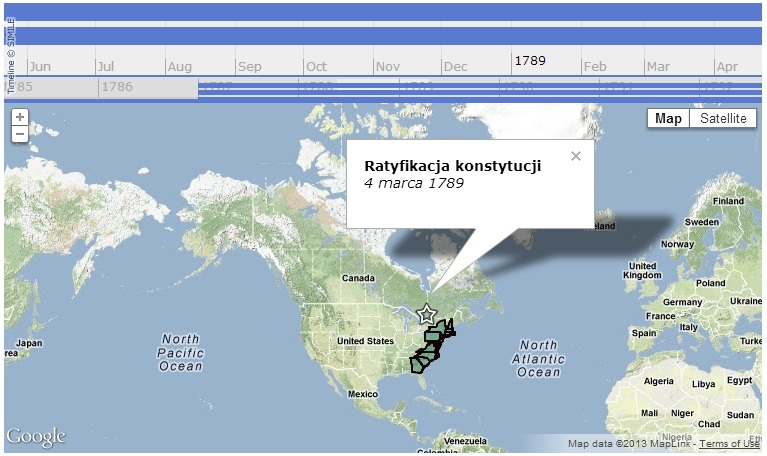
\includegraphics[width=100mm]{ge/st1.jpg}
  \caption{Rok 1789.}
  \label{fig:st1}
\end{figure}

Kolejny rysunek ukazuje aktualny stan granic. Widać że utrzymuje się on od 1959 roku.

\begin{figure}[H]
  \centering
    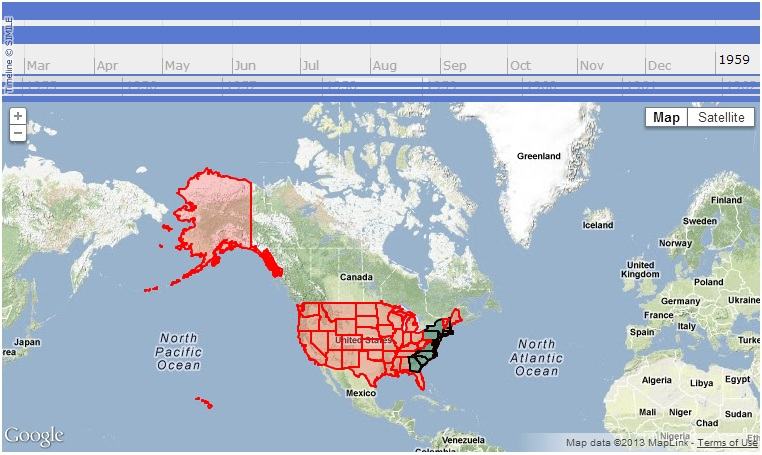
\includegraphics[width=100mm]{ge/st3.jpg}
  \caption{Rok 1959.}
  \label{fig:st3}
\end{figure}

\section{Granice Polski i Rzeczpospolitej Obojga Narodów}
\label{sec:usahistory}

Kolejny przykład przedstawia możliwość zmiany rodzaju danych w zależności od stopnia przybliżenia. Rysunek \ref{fig:po1} przedstawia granice wytyczone przy pomocy funkcji tworzącej linie bezier-a. Przy tak dużym oddaleniu szczegóły rysunku nie są widoczne, nie można przekazać wielu szczegółów.

\begin{figure}[H]
  \centering
    \includegraphics[width=100mm]{ge/polska-teraz.png}
  \caption{Polska obecnie.}
  \label{fig:po1}
\end{figure}

W prosty sposób można określić ogólne granice w dowolnym punkcie w czasie. Poniższy rysunek przedstawia wynik obszaru który został określony przez 105 punktów.

\begin{figure}[H]
  \centering
    \includegraphics[width=100mm]{ge/polska-ron.png}
  \caption{Polska w roku 1691.}
  \label{fig:po2}
\end{figure}

W celu dostarczenia większej ilości informacji, możliwe jest załączenie pliku graficznego, w tym przypadku jest to zdjęcie mapy która przedstawia dokładny obszar Rzeczpospolitej Obojga Narodów. Jeszcze bliższe przybliżenie pozwali na odczytanie nazw miejscowości i obszarów geograficznych.

\begin{figure}[H]
  \centering
    \includegraphics[width=100mm]{ge/polska-ron-map.png}
  \caption{Rzeczpospolita Obojga Narodów, mapa.}
  \label{fig:po3}
\end{figure}
